\documentclass[12pt, a4paper]{article}
\usepackage[utf8]{inputenc}
\usepackage[czech]{babel}
\usepackage[T1]{fontenc}
\usepackage{graphicx}
\usepackage{amsmath, amssymb, amsthm}
\usepackage[margin=2.5cm]{geometry}
\usepackage{url}
\begin{document}

\begin{titlepage}
    \begin{center}
        {\large {Přírodovědecká fakulta}} \\
        \vspace{0.2cm}
        {\large Univerzita Karlova}
        
        \vspace{1.5cm}
        
\includegraphics[width=0.5\linewidth]{img/PrFUK_strom_digital_cerna.png} 
        \vfill{}
        
        {\huge\bfseries Generalizace budov} \\
        \vspace{0.5cm}
        {\large {Algoritmy počítačové kartografie}} \\
        \vfill
        
        \begin{center}
            \large Teodor Sorokáč \\
        \end{center}
        \vfill{}

        \begin{center}
            \ 2. N-GKDPZ \\
            \ Praha 2026
        \end{center}
        
    \end{center}
\end{titlepage}

\newpage
\section{Zadání}

\vspace{5mm}
\subsection*{\textbf{Úloha č. 2: Generalizace budov LOD0}}

\vspace{3mm}
\noindent\textit{Vstup: množina budov \ $B = \{B_i\}_{i=1}^{n}, \textit{ budova } B_i = \{P_{i,j}\}_{j=1}^{m}$}\
\vspace{3mm}

\noindent\textit{Výstup: $G(B_i)$}
\vspace{3mm}

\noindent Ze souboru načtěte vstupní data představovaná lomovými body budov a proveďte generalizaci budov do úrovně detailu LOD0. Pro tyto účely použijte vhodnou datovou sadu, např. ZABAGED, testování proveďte nad třemi datovými sadami (historické centrum města, izolovaná zástavba).
\vspace{3mm}

\noindent Pro každou budovu určete její hlavní směry metodami:
\vspace{3mm}
\begin{itemize}
    \item Minimum Area Enclosing Rectangle
    \item PCA
\end{itemize}
\vspace{3mm}

\noindent U první metody použijte některý z algoritmů pro kontrukci konvexní obálky. Budovu při generalizaci do úrovně LOD0 nahraďte obdélníkem orientovaným v obou hlavních směrech, se středem v těžišti budovy, jeho plocha bude stejná jako plocha budovy. Výsledky generalizace vhodně vizualizujte.
\vspace{3mm}

\noindent Otestujte a provnejte efektivitu obou metod s využitím hodnotících kritérií. Pokuste se rozhodnout, pro které tvary budo dávají metody nevhodné výsledky, a pro které naopak poskytují vhdnou aproximaci. 

\vspace{1cm}
\subsection*{\textbf{Hodnocení:}}

\begin{center}
\resizebox{\textwidth}{!}{
\begin{tabular}{|l|c|}
\hline
\textbf{Krok}                                                                                  & \textbf{Hodnocení} \\ [0.5ex]  \hline\hline
\rule{0pt}{3ex} Generalizace budov metodami Minimum Area Enclosing Rectangle a PCA.                                    &  15b              \\ \hline
\rule{0pt}{3ex}\textit{Generalizace budov mnetodou Longest Edge.}                    & \textit{+5b}    \\ \hline
\rule{0pt}{3ex}\textit{Generalizace budov metodou Wall Average.} & \textit{+8b}    \\ \hline
\rule{0pt}{3ex}\textit{Generalizace budov metodou Weighted Biscetor.}   & \textit{+10b}    \\ \hline
\rule{0pt}{3ex}\textit{Implementace další metody konstrukce konvexní obálky.} & \textit{+5b} \\ \hline
\rule{0pt}{3ex}\textit{Ošetření singulárních případů při generování konvexní obálky.}                    & \textit{+2b}    \\ \hline
\rule{0pt}{3ex}\textit{Načtení vstupních dat ze *.shp.}                    & \textit{+10b}    \\ \hline
\rule{0pt}{3ex}\textbf{Max celkem:} & \textbf{55b} \\ \hline
\end{tabular}
}
\end{center}
\vspace{0.5 cm}

\subsection*{Řešené bonusové úlohy}
V rámci úlohy byly vypracované následující bonusové úlohy: \textit {Generalizace budov mnetodou Longest Edge (5b), Generalizace budov metodou Wall Average (8b), Generalizace budov metodou Weighted Biscetor (10b), Ošetření singulárních případů při generování konvexní obálky (2b), Načtení vstupních dat ze *.shp (10b).}

\newpage
\section{Úvod do problematiky úlohy}
\vspace{5mm}
Generalizace je stěžejní proces v kartografii. Cílem je zjedodušení objektů v závislosti na jejich velikosti a měřítku mapy. Při oddalování se objekty zkreslují a zjednodušují. 
\vspace{3mm}

\noindent Generalizace budov zahrnuje různé aspekty, mezi které patří zjednodušení geometrie, seskupování objektů, které se nachází blízko sebe, změna velikosti a polohy a také výběr důležitých objektů, které jsou důležitější pro zobrazení než jiné. Zároveň je důležité zachování jejich charakteristických rysů.  
\vspace{3mm}

\noindent Pro automatizaci generalizace se používá především algoritmy jako Minimum Area Enclosing Rectangle, Principal Component Analysis, Longest Edge, Weighted Biscetor a Wall Avarege. V rámci úlohy byly zpracovány všechny tyto algoritmy a v následujících kapitolách budou přiblíženy jejich principy. 
\vspace{2cm}


\newpage
\section {Minimum Area Enclosing/Bounding Rectangle}

\vspace{1cm}
Metoda Minimum Area Enclosing/Bounding Rectangle hledá obdélník, který má nejmenší možnou plochu. Hlavním účelem je určení orientace objektu v prostoru. Algoritmus hledá co nejmenší obdélník, který obklopuje množinu vrcholů. Nejprve je vytvořena konvexní obálka, kterou poté otáčíme o úhel $-\sigma$. 
\vspace{1cm}
$$P_0 = R(-\sigma)P \Rightarrow
\begin{bmatrix} x_r \\ y_r \end{bmatrix} =
\begin{bmatrix} \cos(-\sigma) & -\sin(-\sigma) \\ \sin(-\sigma) & \cos(-\sigma) \end{bmatrix}
\begin{bmatrix} x \\ y \end{bmatrix}$$
\vspace{1.5cm}

\noindent Po kaýdém otočení je vyhodnocován nejlépe vytvořený obdélník s nejmenší plochou. Poté co projde všechny úhly, tak se otočí zpět o úhel $-\sigma$ do původní pozice. Postup pro určení orientace je totožný u ostatních metod generalizace. 

\newpage
\section {Principal Component Analysis (PCA)}
\vspace{1cm}
Metoda PCA je statický přístup pro generalizaci objektů. Je zde využito singulární rozklad kovarianční matice C:

\vspace{1cm}
$$C=U \Sigma V^T, \begin{bmatrix} c_{11} & c_{12} \\ c_{21} & c_{22} \end{bmatrix} =
\begin{bmatrix} u_{11} & u_{12} \\ u_{21} & u_{22} \end{bmatrix}
\begin{bmatrix} \sigma_1 & 0 \\ 0 & \sigma_2 \end{bmatrix}
\begin{bmatrix} v_{11} & v_{12} \\ v_{21} & v_{22} \end{bmatrix}^T$$
\vspace{1cm}

Kde C představuje kovarianční matici definovanou jako: 

$$C= \begin{bmatrix} C(A, A) & C(A, B) \\ C(B, A) & C(B, B) \end{bmatrix},
C(A, B)=\frac{1}{n-1} \sum\limits_{i=1}^{n} (A_i-\mu_A)(B_i-\mu_B)$$
\vspace{1cm}

\noindent Matice $U$ a $V$ jsou ortogonální matice, což v praxi znamená, že jejich sloupcové vlastní vektory jsou na sebe kolmé a mají jednotkovou velikost. Matice $\Sigma$ je pak diagonální matice, která má na hlavní diagonále čtverce velikostí vlastních vektorů (odmocniny vlastních čísel $\lambda$):
\vspace{1cm}

$$U=V=\begin{bmatrix} \cos \sigma & -\sin \sigma \\ \sin \sigma & \cos \sigma \end{bmatrix}$$
\vspace{1cm}

$$\Sigma=\begin{bmatrix} \sigma_1 & 0 \\ 0 & \sigma_2 \end{bmatrix}=
\begin{bmatrix} \sqrt{\lambda_1} & 0 \\ 0 & \sqrt{\lambda_2} \end{bmatrix}$$
\vspace{1cm}

\noindent Metoda PCA je velmi efektivní metodou, která bere v potaz rozložení všech vrcholů objektu a nevyužívá pouze konvexní obálku.
\vspace{1cm}

\newpage
\section {Longest Edge}

\vspace{1cm}
Metoda Longest Edge je jednou z nejjednodušších metod pro generalizaci. Stejně jako první metoda využívá konvexní obálku, která obepíná vrchovly objektu. Pro určení směru však využívá pouze informace nejdelší strany. Tento způsob může být problémový u jistých objektů, kde nejdelší strana nemusí odpovídat pravé velikosti objektu a jeho orientace. Pro objekty tvaru obdélníku je však tato metoda velmi dobře využitelná. 

\vspace{1cm}
\noindent Hlavní úhel $\sigma$ je určen směrovým úhlem nejdelší hrany mezi vrcholy $P_i$ a $P_{i+1}$:
\vspace{1cm}
$$\sigma = \arctan \left( \frac{y_{i+1} - y_i}{x_{i+1} - x_i} \right)$$
\vspace{1cm}

\newpage
\section {Wall Average}

\vspace{1cm}
Algoritmus Wall Average je variace předchozí metody, avšak je doplněn o výpočet, který zahrnuje orientaci všech hran objektu. Každé hraně je přiřazena váha, stejně jako u váženého průměru, na základě její délky. Důležitým krokem je modulace vzhledem k pravému úhlu, tím zajišťujeme, aby protilehlé hrany neovlivňovaly výpočty váženého průměru. 

\vspace{1cm}
\noindent Nejprve se stanoví odchylky směrnic hran $\sigma_i$ od referenčního směru $\sigma'$:
\vspace{1cm}
$$ \Delta\sigma_i = |\sigma_i - \sigma'| $$
\vspace{1cm}


\noindent V dalším kroce se vypočítá násobek prvního úhlu.
\vspace{1cm}
$$ k_i = \text{round} \left( \frac{2 \Delta \sigma_i}{\pi} \right) $$
\vspace{1cm}

\noindent Poté se určí orintovaný zbytek po dělení.
\vspace{1cm}
$$ r_i = \Delta\sigma_i - k_i \frac{\pi}{2} $$
\vspace{1cm}

\noindent Finální směr $\sigma$ je definován jako vážený průměr zbytků, kde vahou jsou délky stran.
\vspace{1cm}
$$ \sigma = \sigma' + \frac{\sum_{i=1}^{n} (r_i s_i)}{\sum_{i=1}^{n} s_i} $$
\vspace{1cm}

\newpage
\section {Weighted Bisector}
\vspace{1cm}
Metoda Weighted Bisector identifikuje hlavní směr analýzou os souměrnosti nebo-li bisektorů, které jsou mezi protilehlými hranami objektu. Pro každou nalezenou dvojici hran s orientacemi $\alpha_{j,1}$ a $\alpha_{j,2}$ se určí úhel jejich bisektoru $\beta_j$:
\vspace{1cm}
$$ \beta_j = \frac{\alpha_{j,1} + \alpha_{j,2}}{2} $$
\vspace{1cm}

\noindent Každý bisektor je vážen významem příslušných segmentů a nejčasteji jejich délkou $w_j$:
\vspace{1cm}
$$ \sigma = \frac{\sum (w_j \cdot \beta_j)}{\sum w_j} $$
\vspace{1cm}

\noindent Algoritmus efektivně eliminuje vliv drobných hran a lépe tak vystihne generalizovanou geometrii objektu. 

\newpage
\section {Aplikace}
\vspace{5mm}
Aplikace se otevře spuštěním skriptu MainForm.py a otevře se interaktivní okno, ve polygon. Nad lištou tlačítek se nachází nabídka tří možností: \textit {File}, \textit {Simplify} a \textit {View}. Po rozkliknutí záložky \textit {File} se nabídne možnost vložení vlastní polygonové vrstvy z počítače uživatele. Tlačítko \textit {Simplify} po rozkliknutí nabídne uživateli několik možností pro generalizaci polygonu. Záložka \textit {View} nabídne uživateli dvě možnosti a to jedna pro smazání výsledku \textit{clear result} (typ generalizace) a možnost \textit{Clear all}, která smaže vše i s polygonem či polygonovou vrstvou. Dále je okno doplněno o záložku \textit {Open}, které nabízí možnost vložení souboru ve formátu shapefile, nad kterým lze provést zpracované způsoby generalizace objektu: \textit {Minimum Area Bounding Rectangle, PCA, Longest Edge, Wall Average} a \textit {Weighted Bisector}. Dále se na liště nachází opět tlačítka \textbit {clear result} a \textit{clear all}. Posledním tlačítkem \textit{Close application} se interaktivní okno aplikace zavře. 
\vspace{3mm}

\noindent V případě vložené vlastní polygonové vrstvy se velikost zobrazované vrstvy přizpůsobí otevřenému oknu aplikace. 
\vspace{3mm}

\noindent Po spuštění generalizace pomocí libovolné metody se zobrazí červený polygon, který indikuje, jak by generalizace tímto způsobem vypadala. Tlačítkem \textit {clear result} se generalizovaný polygon smaže a lze použít jinou metodu generalizace. Tlačítkem \textit{clear all} se smaže vše a lze nakreslit nový polygon, či vložit jinou polygonovou vrstvu. 
\vspace{1cm}

\begin{figure}[h!]
    \centering
    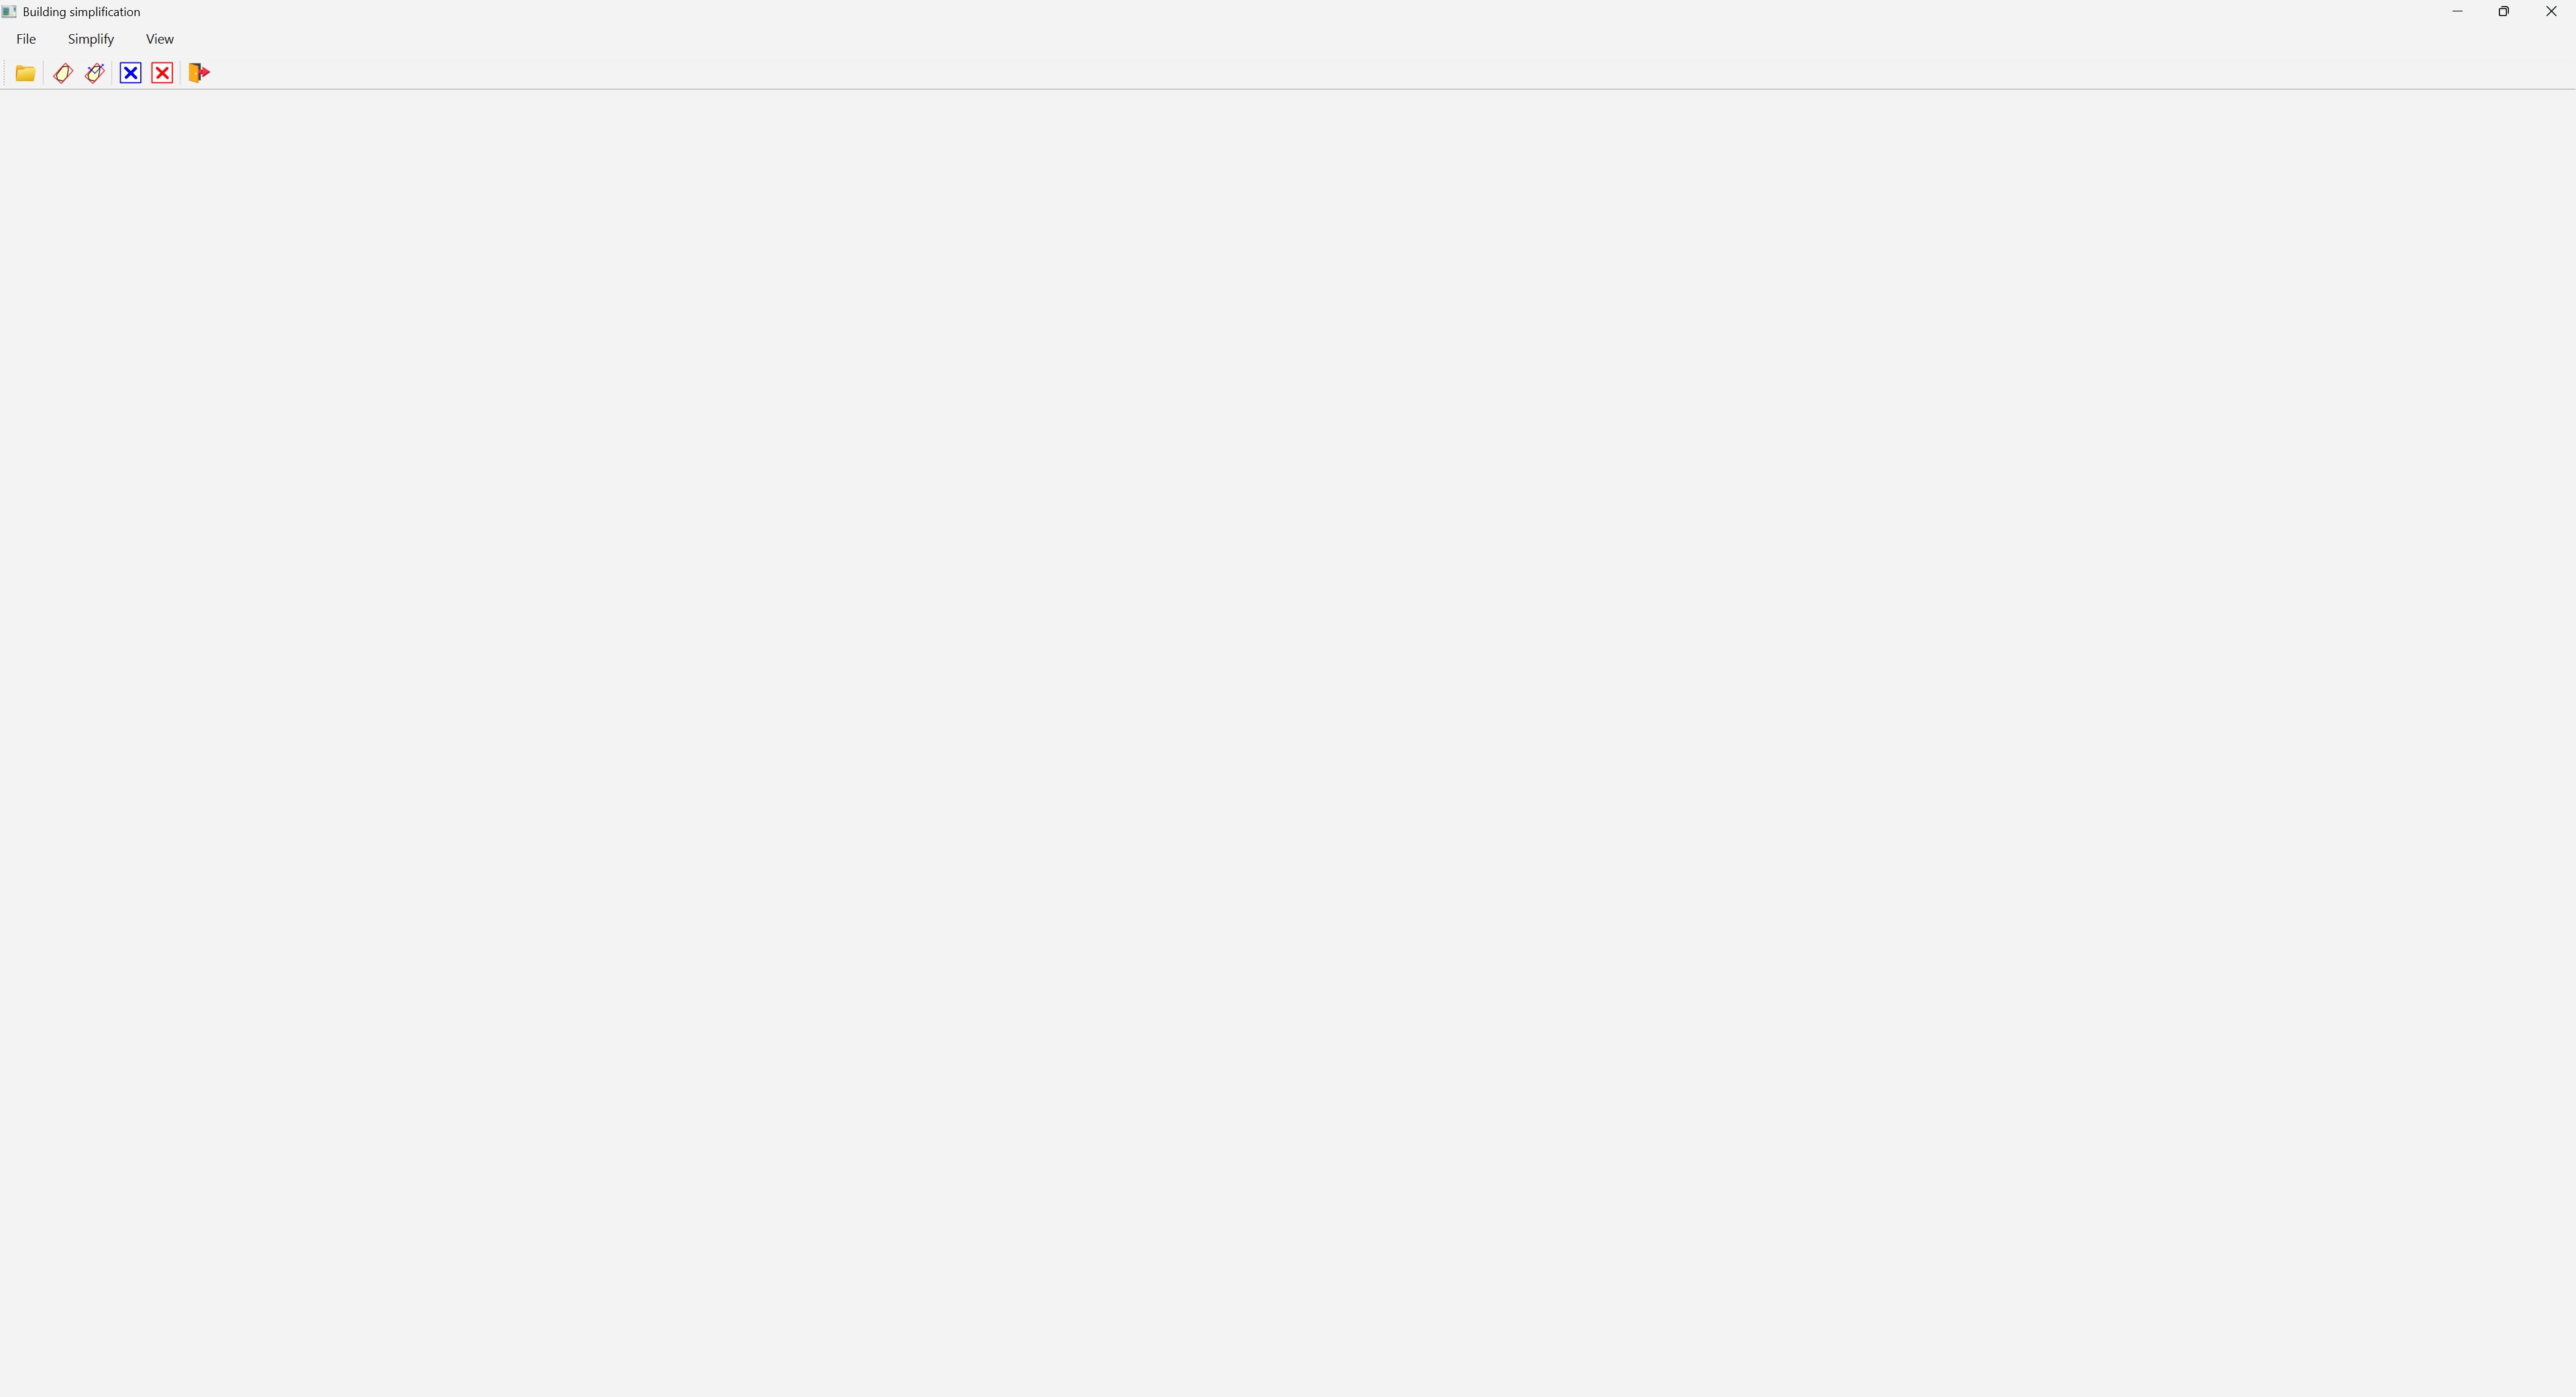
\includegraphics[width=0.5\linewidth]{img/screenshot.jpg}
    \caption{\centering\textit{Uživatelské prostředí aplikace}}
    \label{fig:placeholder}
\end{figure}


\newpage
\section {Dokumentace}
\vspace{5mm}
Úloha byla vypracována v softwaru Visual Studio Code v jazyce Python a obsahuje 3 soubory se skripty, které na sebe odkazují (algorithms.py, draw.py, MainForm.py). Pro zapisování skriptů byl použit formát CamelCase. 
\vspace{5mm}
\subsection*{algorithms.py}
\vspace{3mm}
V tomto souboru byly uloženy následující funkce:
\vspace{3mm}

\begin{itemize}
    \item \textbf{def get2VectorsAngle} - Tato funkce počítá velikost úhlu mezi dvěma zadanými vektory. Ošetření proti dělení nulou. 
    \item \textbf{def createCH} - Funkce vytváří konvexní obálku nad zadaným polygonem nebo polygonovou vrstvou. Vychází z prvního vrcholu a postupně přidává další vrcholy.
    \item \textbf{def createMMB} - Tato funkce vytváří min-max box pro zadaný polygon a zároveň počítá jeho plochu.
    \item \textbf{def rotatePolygon} - Funkce rotuje polygon o zadaný úhel. 
    \item \textbf{def createMBR} - Funkce vyhledává minimální opsaný obdélník kolem konvexní obálky.
    \item \textbf{def getArea} - Funkce počítá plochu zadaného polygonu. 
    \item \textbf{def resizeRectangle} - Funkce upravuje velikost opsaného obdélníku tak, aby jeho plocha odpovídala původní velikosti.
    \item \textbf{def simplifyBuildingMBR} - Funkce generalizuje polygon pomocí metody Minimum Area Bounding Rectangle.
    \item \textbf{def simplifyBuildingPCA} - Funkce generalizuje polygon pomocí metody Principal Component Analysis.
    \item \textbf{def simplifyBuildingLongestEdge} - Funkce generalizuje polygon pomocí metody Longest Edge (podle její nejdelší hrany).
    \item \textbf{def simplifyBuildingWallAverage} - Funkce generalizuje polygon pomocí metody Wall Average (vážený průměr hran).
    \item \textbf{def simplifyBuildingWeightedBisector} - Funkce generalizuje polygon pomocí metody Weighted Bisector. 
\end{itemize}

\newpage
\subsection*{draw.py}
\vspace{3mm}
V tomto souboru byly uloženy následující funkce:
\vspace{3mm}

\begin{itemize}
    \item \textbf{def mousePressEvent} - Funkce určuje souřadnice vrcholů polygonu, na základě kliknutí do plátna aplikace.
    \item \textbf{def paintEvent} - Funkce vykresuje grafiku (polygon, polygonovou vrstvu) na plátno. 
    \item \textbf{def setMBR} - Funkce nastavuje polygon reprezentující MBR. 
    \item \textbf{def setCH} - Funkce nastavuje polygon reprezentující CH.
    \item \textbf{def getBuilding} - Funkce vrací analyzovaná data, pokud byla vložena polygonová vrstva, vrací seznam budov. 
    \item \textbf{def clearResult} - Funkce vymaže generalizovanou vrstvu. 
    \item \textbf{def openFile} - Funkce otevře systémové okno, ve kterém je možnost nahrání vlastní polygonové vrstvy ve formátu *.shp.
    \item \textbf{def geomShapefile} - Funkce vykreslí zvolenou polygonovou vrstvu formátu *.shp do aplikace a polygony zařadí do seznamu. Funkce zajišťuje zpracování vstupní geometrie a upraví ji na souřadnice dle velikosti plátna aplikace. 
    \item \textbf{def clearAll} - Funkce smaže veškerá data na plátně.
    \item \textbf{def setSimplifBuilding} - Funkce ukládá seznam výsledných generalizovaných polygonů a překresluje je, aby se mohl zobrazit další generalizovaný polygon.
\end{itemize}

\newpage
\subsection*{MainForm.py}
\vspace{3mm}
V tomto souboru byly uloženy následující funkce:
\vspace{3mm}

\begin{itemize}
    \item \textbf{def simplifyBuildingPCAClick} - Funkce zavolá generalizační algoritmus metody PCA.
    \item \textbf{def simplifyBuildingMBRClick} - Funkce zavolá generalizační algoritmus metody Minimum Bounding Rectangle.
    \item \textbf{def simplifyBuildingLongestEdgeClick} - Funkce zavolá generalizační algoritmus metody Longest Edge.
    \item \textbf{def simplifyBuildingWallAverageClick} -  Funkce zavolá generalizační algoritmus metody Wall Average.
    \item \textbf{def simplifyBuildingWWeightedBisectorClick} -  Funkce zavolá generalizační algoritmus metody Weighted Bisector.
    \item \textbf{def openFileClick} - Funkce zavolá \textit{def openFile} ve skriptu draw.py pro načtení polygonové vrstvy.
    \item \textbf{def exitClick} - Funkce ukončí aplikaci.
    \item \textbf{def clearResultsClick} - Funkce zavolá metodu \textit{clearResult} ve skriptu draw.py a smaže výsledky.
    \item \textbf{def clearAllClick} - Funkce zavolá metodu \textit{clearAll} ve skriptu draw.py a smaže celé plátno.
\end{itemize}

\newpage
\section{Zhodnocení přesnosti algoritmů}
\vspace{5mm}
Porovnání efektivity a přesnosti algoritmů pro generalizaci budov je zobrazen v následující Tabulce 1. Nejlepších výsledků dosahuje metoda MBR a to ve všech třech datasetech. Neméně dobrých výsledků dosahuje poté algoritmus Longest Edge a PCA. Nejméně vhodný algoritmus se jeví Weighted Bisector, který ve všech datasetech dosahuje nejnižších hodnot. 
\begin{table}[h!]
\centering
\begin{tabular}{|l|c|c|c|}
\hline
\textbf{Algoritmus} & \textbf{BUDOVY (\%)} & \textbf{BUDOVY 2 (\%)} & \textbf{BUDOVY 3 (\%)} \\ \hline
PCA & 87 &  84 & 88  \\ \hline
Min. Bounding Rectangle (MBR) & 91 & 85 & 91  \\ \hline
Longest Edge & 91 & 83 & 91  \\ \hline
Wall Average & 91 & 80 & 90  \\ \hline
Weighted Bisector & 86 & 77 & 83  \\ \hline
\end{tabular}
\caption{Srovnání shody výsledků metod s původními datasety (překryvu v \%)}
\end{table}

\newpage
\section*{Seznam literatury}
\vspace{5mm}
\noindent BAYER, T. (2026): Konvexní obálky. Prezentace pro přednášku předmětu Algoritmu počítačové kartografie, Katedra aplikované geoinformatiky  a kartografie, Přírodovědecká a fakulta UK [cit. 4. 5. 2026].
\vspace{3mm}

\end{document}